\documentclass{article}

%语言页面以及字体设置
\usepackage{ctex}
\usepackage{a4}
\usepackage{indentfirst}
\setlength{\parindent}{2em}
\usepackage{xeCJK}
\usepackage{fontsize}
\usepackage{subfigure}
\usepackage{subcaption}

%其他宏包
\usepackage{amsmath}
\usepackage{graphicx}
\usepackage[a4paper, left=2.5cm, right=2.5cm, top=2.5cm, bottom=2.5cm]{geometry}

%插入代码
\usepackage{listings,matlab-prettifier}
\lstset{style=Matlab-editor,numbers = left,frame = single,}


\title{Bicycle Model Handling Simulation}
\author{葛逸凡 3210103331 使用Matlab R2022b}
\date{\today}

\begin{document}

\maketitle

\section{simulink模型搭建}

根据书本公式(5-9):

$$
\begin{cases}
\dot{v} = ((k_1+k_2)\frac{v}{n}+\frac{1}{u}(ak_1-bk_2)\omega_r -k_1\delta)/m-u\omega_r \\
\dot{\omega_r}=((ak_1-bk_2)\frac{v}{u}+\frac{1}{u}(a^2k_1+b^2k_2)\omega_r-ak_1\delta)/I_z
\end{cases}
$$    

使用simulink中的Matlab function模块,编写出$\dot{v},\dot{\omega_r}$关于$v,\omega_r,\delta,u$的方程。

\begin{figure}[h]
    \centering
    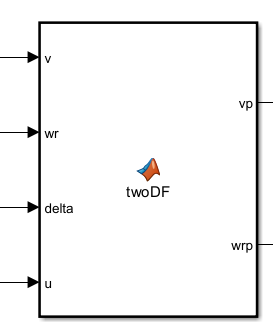
\includegraphics[width=2.5cm]{figure/fcn.png}
    \caption{Matlab function 模块}
    \label{matlabfcn}
\end{figure}

其中$v$和$\omega_r$分别由$\dot{v}$和$\dot{\omega_r}$积分得到。在第五章的特定条件下,汽车$x$轴的前进速度$u$视为不变,$\delta$手动设置以研究不同操作下车辆模型的响应。最终线性二自由度汽车simulink模型如下图所示

\begin{figure}[h]
    \centering
    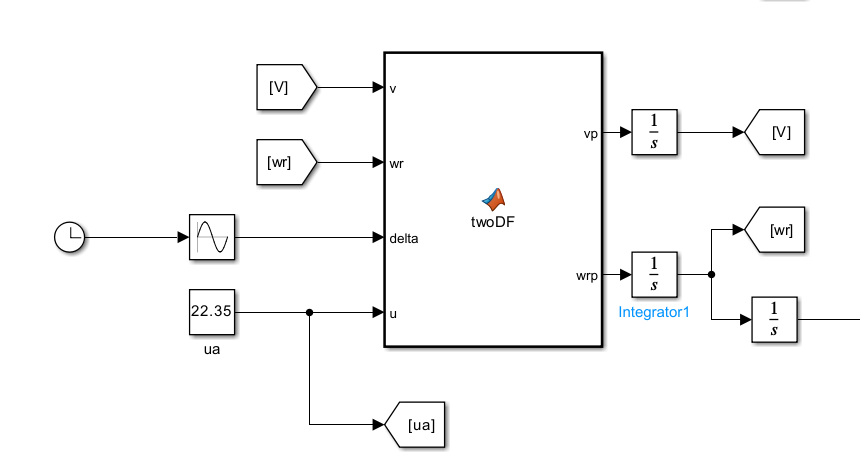
\includegraphics[width=5.5cm]{figure/2DF.png}
    \caption{线性二自由度汽车模型}
    \label{2DF}
\end{figure}



\section{习题作答}

\noindent \bf{(1)稳定性因素$K$、特征车速$u_{ch}$:}

$$
    K = \frac{m}{L^2}(\frac{a}{k_2}-\frac{b}{k_1})=\frac{1818.2}{3.048^2}(\frac{1.463}{-110185}-\frac{1.585}{-62618})=2.355\times10^{-3} s^2/m^2
$$

$$
    u_{ch} = \sqrt{1/K} = \sqrt{1/(2.355\times10^{-3})} = 20.6 m/s
$$

\noindent \bf{(2)稳态横摆角速度增益曲线$\frac{\omega_r}{\delta})_s-u_a$}

由式(5-11)可知,

$$
    \frac{w_r}{\delta}\big)_s = \frac{u/L}{1+Ku^2}
$$

因此设计Matlab程序:
\begin{lstlisting}[language=Matlab]
    %上题求得的稳定性因数
    K = 2.355*10^(-3);
    %车身长度
    L = 3.048;
    %速度区间设置在1-40m/s
    u = 1:40;
    %横摆角速度增益曲线
    YawRateGain1 = (u/L)./(1+K*u.^2);
    %设置K=0的情况作为对照
    YawRateGain2 = u/L;
    %绘图
    plot(u,YawRateGain1);
    axis([0 40 0 10]);
    hold on
    plot(u,YawRateGain2)
\end{lstlisting}

获得横摆角速度增益曲线如下图所示。

\begin{figure}[h]
    \centering
    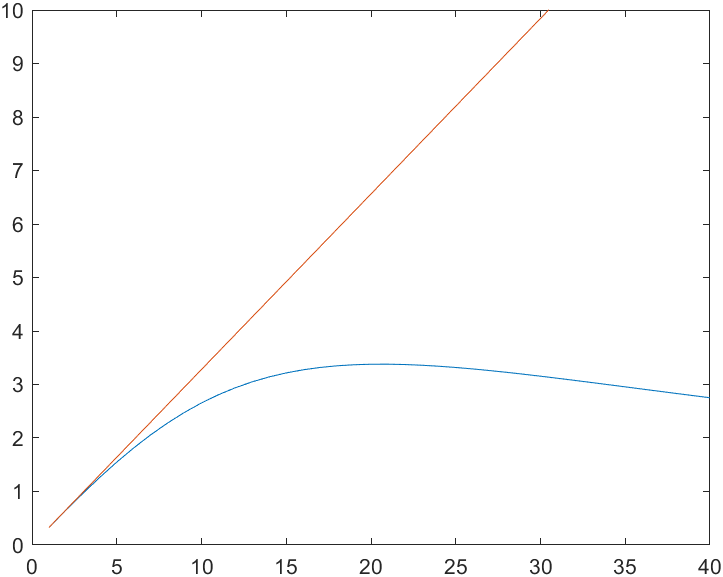
\includegraphics[width=5.5cm]{figure/YRG.png}
    \caption{横摆角速度增益曲线}
    \label{YawRateGainCurve}
\end{figure}

\noindent \bf{(3)车速$u_a=22.35m/s$时的转向灵敏度$\frac{\omega_r}{\delta_{s\omega}}$

根据公式(5-11)计算可得,车速$u_a=22.35m/s$时的稳态横摆角速度增益$\frac{w_r}{\delta})_s=3.37$,
该车的转向系总传动比$i=20$,即$\delta_{s\omega}=i\delta$,所以$\frac{\omega_r}{\delta_{s\omega}}=\frac{\omega_r}{\delta})_s/i=0.1685$

\noindent \bf{(4)静态储备系数S.M.}
由公式(5-17)可得:
$$
    S.M. = \frac{k_2}{k_1+k_2}-\frac{a}{L} = \frac{-110185}{-62618-110185}-\frac{1.463}{3.048} = 0.157
$$
S.M.为正值,汽车具有不足转向特性。

\noindent \bf{(5)侧向加速度为0.4g时的前、后轮侧偏角绝对值之差$\alpha_1-\alpha_2$与转弯半径的比值$R/R_0(R_0=15m)$}
由公式(5-13)可得,
$$
\alpha_1-\alpha_2 = K\times a_yL = 28.13\times10^{-3} rad 
$$

$$
\begin{gathered}
    R_0 = L/\delta = 15m, \\
    \delta = 0.2032 rad \\
    R = \frac{L}{\delta - (\alpha_1-\alpha_2)} = \frac{3.048}{0.2032-0.02813} = 17.41m\\
    \frac{R}{R_0} = \frac{17.41}{15} = 1.16;
\end{gathered}
$$

\noindent \bf{(6)车速$u=30.56m/s$时,瞬态相应的横摆角速度波动的固有(圆)频率$\omega_0$、阻尼比$\zeta$、反应时间$\tau$与峰值反应时间$\epsilon$}

由公式(5-34),(5-35),(5-36),(5-37)得:
$$
\begin{gathered}
    \omega_0 = \frac{L}{u}\sqrt{\frac{k_1k_2}{mI_z}(1+Ku^2)} = 4.62 \\
    \zeta = \frac{-m(a^2k_1+b^2k_2)-I_Z(k_1+k_2)}{2L\sqrt{mI_Zk_1k_2(1+Ku^2)}} = 0.589\\
    \tau = -\frac{arctan[\frac{\sqrt{1-\zeta^2}}{(-\frac{mua}{Lk_2}\omega_0-\zeta)}]}{\omega_0\sqrt{1-\zeta^2}} = 0.2586s\\
    \epsilon = \frac{arctan(\frac{\sqrt{1-\zeta^2}}{\zeta})}{\omega_0\sqrt{1-\zeta^2}}+\tau = 0.467s
\end{gathered}
$$


\section{使用Simulink模型进行进一步探究}

\subsection{完善simulink模型}

为了更加直观地感受车辆的操作响应,为simulink模型添加大地坐标系下X、Y坐标的计算。由书本图5-23及图5-24可清晰得知大地坐标系下车辆在
X轴和Y轴的速度分量与车辆的质心速度的关系分别为:
$$
\begin{cases}
    v_X = v_1 cos(\beta+\phi)\\
    v_Y = v1 sin(\beta+\phi)
\end{cases}
$$
式中$\beta$为质心侧偏角,可以由$arctan(v/u)$获得;$\phi$为车辆横摆角,可以通过横摆角速度积分获得。
完善后的simulink模型如下图所示:

\begin{figure}[h]
    \centering
    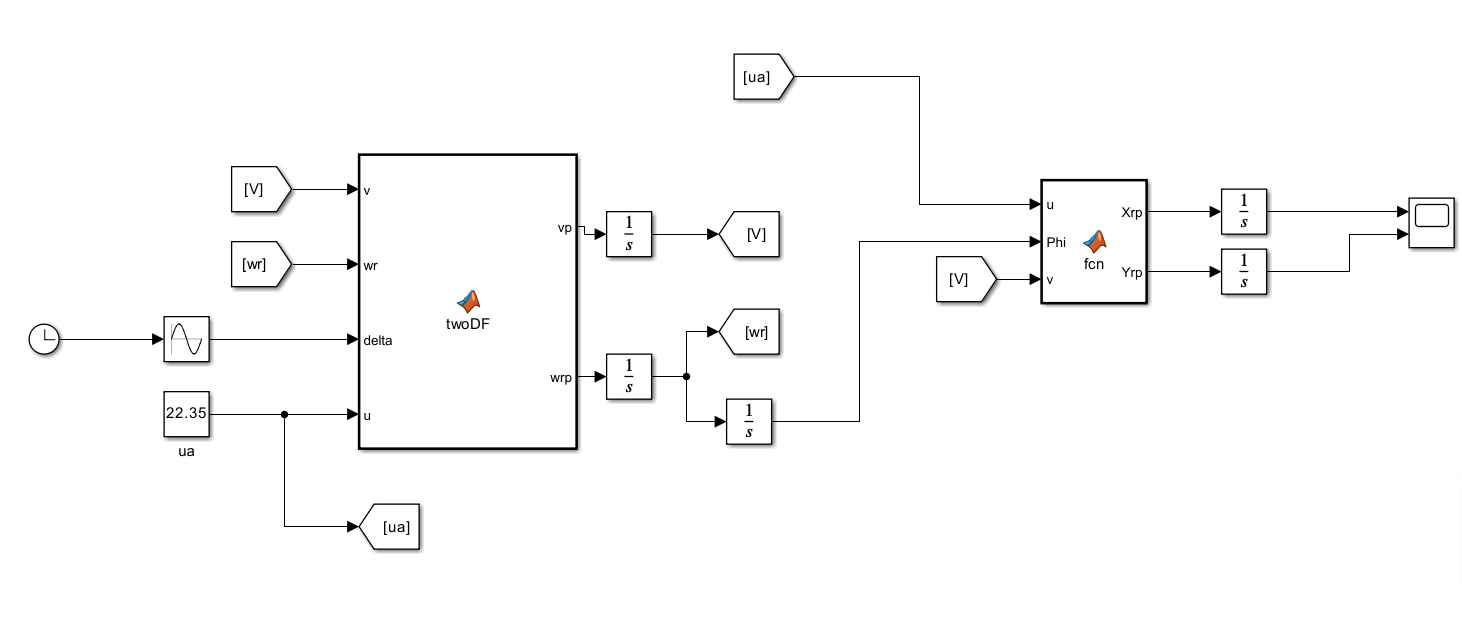
\includegraphics[width=10cm]{figure/final.png}
    \caption{带路径计算的simulink模型}
    \label{simulinkFinal}
\end{figure}

设定前轮转角在-30°-30°范围内以正弦规律转动,得到的车辆路径如图5所示:

\begin{figure}[htbp]
    \centering
    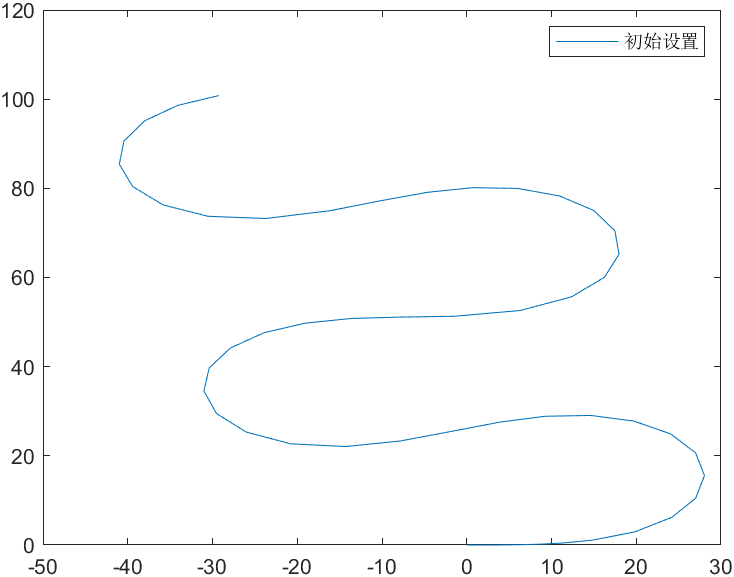
\includegraphics[width=5.5cm]{figure/origin.png}
    \caption{正弦波输入的车辆路径}
    \label{originpath}
\end{figure}

\subsection{改变车速}
设置车速分别为$10m/s,20m/s,30m/s$,运行时间为50s,车辆路径如图6所示:
\begin{figure}[htbp]
    \centering
    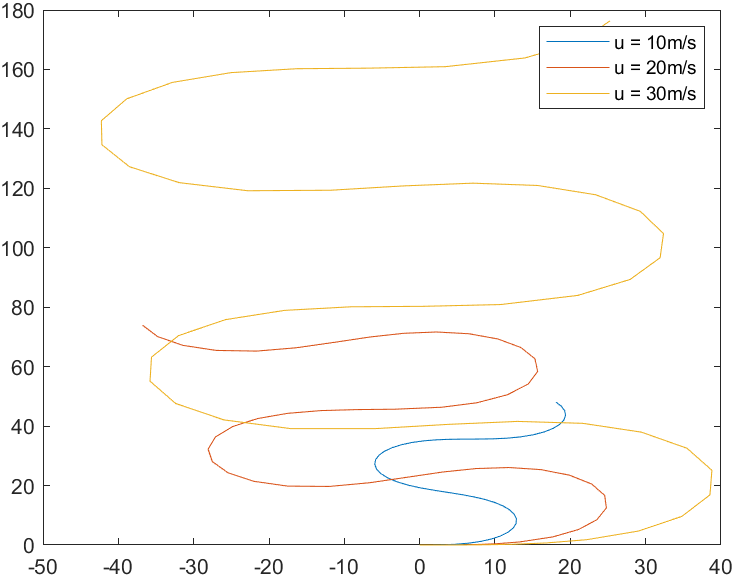
\includegraphics[width=5.5cm]{figure/velocity.png}
    \caption{不同车速下的车辆路径}
    \label{velocity}
\end{figure}

\subsection{改变车辆质量及转动惯量}
设置质量m分别为$1000kg,1818.2kg,2000kg$,转动惯量在保持$m=1818.2kg$时改变为$3000,4500kg\cdotm^2$时,车辆路径如图7所示:
\begin{figure}[htbp]
    \centering
    \subfigure[不同质量下的车辆路径]{
        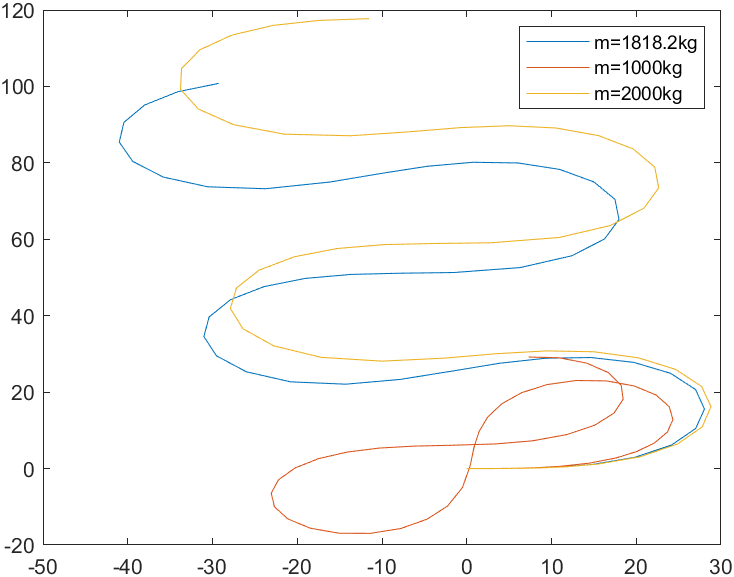
\includegraphics[width=5.5cm]{figure/mass.png}
    }
    \subfigure[不同转动惯量下的车辆路径]{
        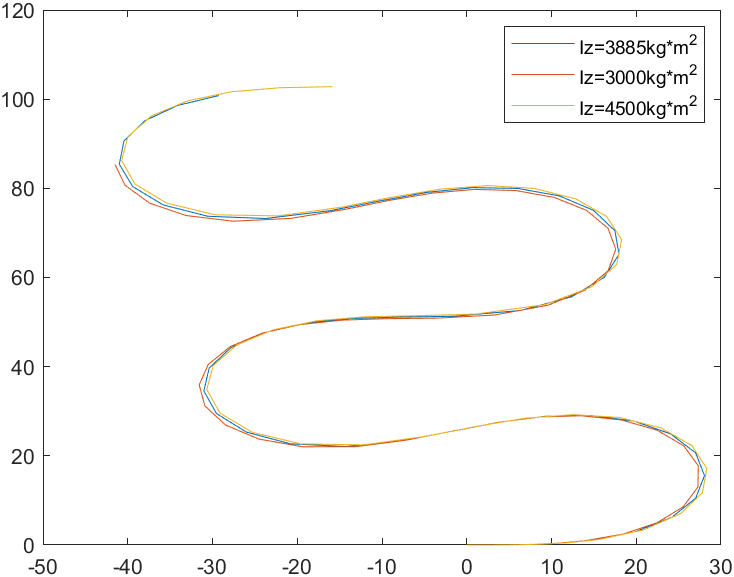
\includegraphics[width=5.5cm]{figure/Iz.png}
    }
    \caption{不同质量、转动惯量下的车辆路径}
    \label{massIz}
\end{figure}

可见质量会影响车辆的操作稳定性,而转动惯量的影响并不明显,主要原因是此时仅仅改变了车辆的转动惯量,事实上转动惯量改变时车辆的其他参数也会发生变化,因此此时研究的转动惯量对车辆操作响应的影响意义不大。

\subsection{改变车辆前轴后轴长度分配以及侧偏刚度}
使车辆前轴长于后轴,得到的车辆路径如图8(a)所示。
\begin{figure}[htbp]
    \centering
    \subfigure[不同前后轴长度分配下的车辆路径]{
        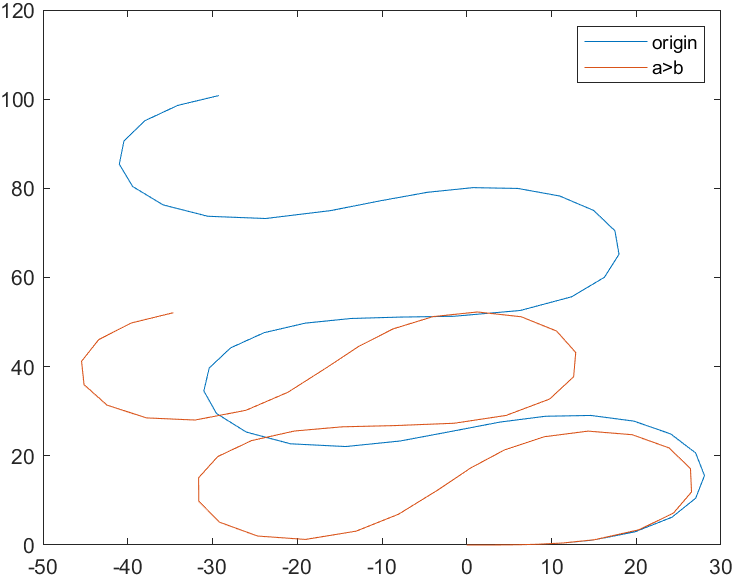
\includegraphics[width=5.5cm]{figure/length.png}
    }
    \subfigure[不同前后侧偏刚度下的车辆路径]{
        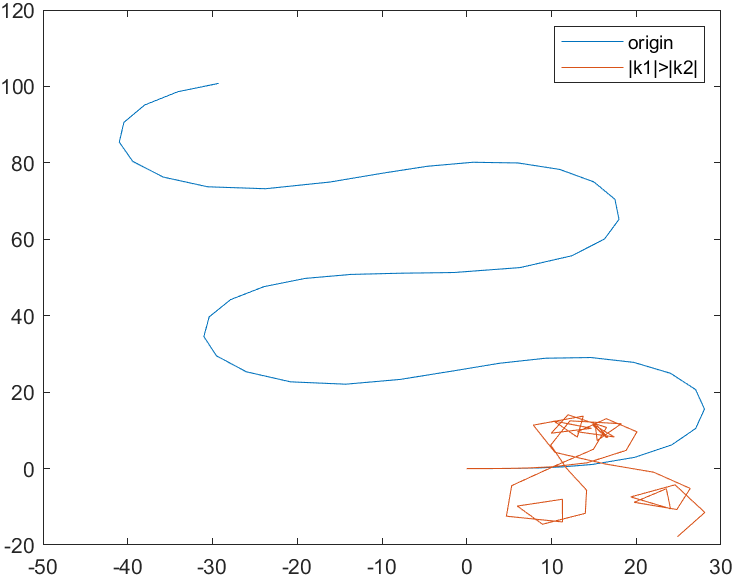
\includegraphics[width=5.5cm]{figure/k.png}
    }
\end{figure}

同理使前轮侧偏刚度的绝对值大于后轮侧偏刚度的绝对值,得到车辆路径如图8(b)所示。可见,当车辆前轴长度大于后轴或者前轮侧偏刚度大于后轮时,都会使车辆趋于过度转向,使操作响应变得不稳定。



\end{document}
